\pstart 
[92 r\textsuperscript{o}] \textso{Gerick. lib. 6. cap. 6.}\edtext{}{\lemma{\textso{6.}}\Bfootnote{\textsc{O. v. Guericke, }\cite{00055}a.a.O., S.~202.}} Solis celerrima gyratio  etiam oculis videri potest, maxime Telescopio\protect\index{Sachverzeichnis}{telescopium}  ut ait Rheita\protect\index{Namensregister}{\textso{Schyrl} (Rheita),  Anton Maria 1597\textendash 1660} lib. 4. c. 1.\edtext{}{\lemma{1.}\Bfootnote{\textsc{A. M. Schyrl, }\cite{00129}\textit{Oculus Enoch et Eliae}, Antwerpen 1645, S.~175f.}} Sol optimo Telescopio\protect\index{Sachverzeichnis}{telescopium} 15 pedum vitris coloratis (sed vide ut  sint duo colorata convexa\protect\index{Sachverzeichnis}{vitrum!convexum}) inspectus instar  continue ebullientis et ferventissimi aeris  flammaeque lucidissimae sese continue in gyrum reciprocantis apparet. (+ Nota quae  de templo S. Nicaesii Lugduni\protect\index{Ortsregister}{Lyon (Lugdunum)} et alibi de Bononiensi S. Petri puto Ricciolus\protect\index{Namensregister}{\textso{Riccioli} (Ricciolus), Giovanni Battista 1598\textendash 1671} +) Aurum\protect\index{Sachverzeichnis}{aurum} ipsum liquefactum se centraliter movet.\pend \pstart \textso{Cap. 7.}\edtext{}{\lemma{7.}\Bfootnote{\textsc{O. v. Guericke}, \cite{00055}a.a.O., S.~203.\protect\rule[0cm]{1cm}{0cm}
}} \textit{Corpora Mundana  sunt Solaria, Planetaria, Lunaria.}  (+ Rectius fixae\protect\index{Sachverzeichnis}{stella!fixa}, Planetae\protect\index{Sachverzeichnis}{planeta}, Sociae. +) Lunaria non circumferuntur a sole\protect\index{Sachverzeichnis}{sol}  ob parvitatem, non proportionalem  distantiae ad impetum recipiendum; sed  a planetae\protect\index{Sachverzeichnis}{planeta} propinquo. (+ Nota Cometam\protect\index{Sachverzeichnis}{cometa} debere rapi cum terra\protect\index{Sachverzeichnis}{terra} ex  hypothesi autoris, quod non facit; si Cometa\protect\index{Sachverzeichnis}{cometa} est effluvium nostrae terrae\protect\index{Sachverzeichnis}{terra}, neque  enim excessit Lunarem regionem  ergo deberet a terra\protect\index{Sachverzeichnis}{terra} circumagi non  minus quam luna\protect\index{Sachverzeichnis}{luna}, nisi dicas nimis  rarum \edtext{et tenue}{\lemma{et}\Afootnote{ \textit{ (1) }\ parvum \textit{ (2) }\ tenue \textit{ L}\protect\rule[0cm]{9cm}{0cm}
}} ejus corpus  quam ut impetum impressum\protect\index{Sachverzeichnis}{impetus!impressus} accipiat. +)\pend
   \begin{center}
   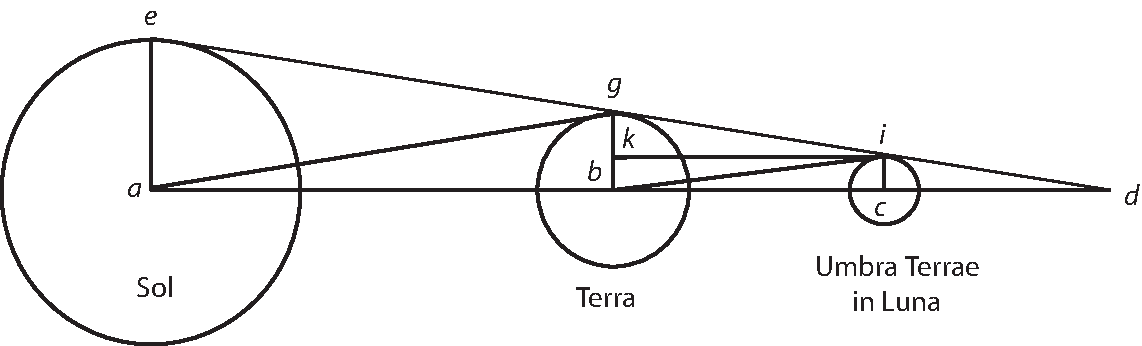
\includegraphics[width=0.8\textwidth]{images/LH35_14_2_92r1}
   \\\textit{[Fig. 5]} \\%\caption{Bildbeschreibung}
    \end{center}
 \pstart \textso{Cap. 9.}\edtext{}{\lemma{\textso{9.}}\Bfootnote{\textsc{O. v. Guericke}, \cite{00055}a.a.O., S.~206\textendash208.}} Supposito diametro solis\protect\index{Sachverzeichnis}{sol} apparente $30\hspace{-6pt}\raisebox{9pt}{,}\protect\hspace{4pt}$ min. et umbrae terrae\protect\index{Sachverzeichnis}{terra}  apparens diameter 80. et diameter lunae\protect\index{Sachverzeichnis}{luna} apparens $30\hspace{-6pt}\raisebox{9pt}{,}\protect\hspace{4pt}$ min. rejectisque perigaeis\protect\index{Sachverzeichnis}{perigaeum} et Apogaeis\protect\index{Sachverzeichnis}{apogaeum}, assumtisque his 4 datis  cum Ptolemaeo\protect\index{Namensregister}{\textso{Ptolemaeus,} Claudius v. Alexandria 85?\textendash 165?}\edtext{}{\lemma{cum}\Bfootnote{Guericke bezieht sich auf \textsc{G. Riccioli}, \cite{00086}a.a.O., S.~106.}}, \textit{hoc modo prout communiter  et in summa in }\textit{meridiano}\protect\index{Sachverzeichnis}{meridianus}\textit{ }\textit{astri}\protect\index{Sachverzeichnis}{astrum}\textit{ elevatione reperiuntur semidiametris tam $\astrosun$ quam $\rightmoon$ apparentibus $15\hspace{-6pt}\raisebox{9pt}{,}\protect\hspace{4pt}$. min. }\textit{Lunae}\protect\index{Sachverzeichnis}{luna}\textit{  distantia a centro }\textit{terrae}\protect\index{Sachverzeichnis}{terra}\textit{ 64  semidiam. }\textit{terrae}\protect\index{Sachverzeichnis}{terra}\textit{ apparente in }\textit{luna}\protect\index{Sachverzeichnis}{luna}\textit{ temp. }\textit{Eclip.}\protect\index{Sachverzeichnis}{eclipsis}\textit{ $40\hspace{-6pt}\raisebox{9pt}{,}\protect\hspace{4pt}$ min.} Primo in $\bigtriangledown$ Rectangulo, \textit{ibc} angulus \textit{b} semidiameter umbrae terrae\protect\index{Sachverzeichnis}{terra} $40\hspace{-6pt}\raisebox{9pt}{,}\protect\hspace{4pt}$. min. et latus \textit{bc} distantia lunae\protect\index{Sachverzeichnis}{luna} a terra\protect\index{Sachverzeichnis}{terra} 64. semidiam. terrae\protect\index{Sachverzeichnis}{terra}. Jam \textit{bc} potest intelligi radius centro \textit{b} et \textit{ic}  tangens et \textit{bc} secans, ergo cum supposito radio \textit{bc} 10,000,000. Tangens $40\hspace{-6pt}\raisebox{9pt}{,}\protect\hspace{4pt}$ min. sit 116361.  \edtext{erit supposito radio}{\lemma{erit}\Afootnote{ \textit{ (1) }\ tangente \textit{ (2) }\ supposito radio \textit{ L}}} 64 semidiam. terrae\protect\index{Sachverzeichnis}{terra} seu 55040 mill. erit inquam  tunc \textit{ic} numerus milliarium multiplicatus per tangentem, divisus per radium \edtext{(omisit divisionem)}{\lemma{}\Afootnote{(omisit divisionem) \textit{ erg.} \textit{ L}}} oriri  ait 640,549 (3 miliaria Germanica.  Aufert magnitudo umbrae \textit{ci} a \textit{bg} vera  semidiametra terrae\protect\index{Sachverzeichnis}{terra} aliunde cognita,  restat \textit{kg} 219,549 (3 milliaria in Germ.  Jam in Triangulo Rectang. \textit{gki} nota  sunt latera \textit{gk} nunc inventa, et \textit{ki} distantia Lunae\protect\index{Sachverzeichnis}{luna}, ergo  et angulus \textit{gik}  invenietur  nempe $13\hspace{-6pt}\raisebox{9pt}{,}\protect\hspace{4pt}$ - $42\hspace{-6pt}\raisebox{9pt}{,,}$.  Is angulus idem cum  angulo \textit{eda} quia  lineae \textit{ki} et \textit{bd} sunt parallelae, in quas cadit eadem \textit{cd}.  Jam quaeritur axis coni umbrae seu linea \textit{bd} ubi dices: uti sinus  ang. \textit{d} $13\hspace{-6pt}\raisebox{9pt}{,}\protect\hspace{4pt}$, $42\hspace{-6pt}\raisebox{9pt}{,,}\protect\hspace{4pt}$ ad sinum complementi id est ang. 90 grad. minus $13\hspace{-6pt}\raisebox{9pt}{,}\protect\hspace{4pt}$, $42\hspace{-6pt}\raisebox{9pt}{,,}\protect\hspace{4pt}$  seu 89 grad. $46\hspace{-6pt}\raisebox{9pt}{,}\protect\hspace{4pt}$ min. $18\hspace{-6pt}\raisebox{9pt}{,,}\protect\hspace{4pt}$ sec. sic semidiam. terrae\protect\index{Sachverzeichnis}{terra} 1. ad axem coni  umbrae \textit{db} erit 250,69 (2.) sem. \edtext{terrae\protect\index{Sachverzeichnis}{terra}. Jam si $13\protect\hspace{-6pt}\protect\raisebox{9pt}{,}\protect\hspace{4pt}$, $46\protect\hspace{-6pt}\protect\raisebox{9pt}{,,}\protect\hspace{4pt}$ subtrahantur at ang. \textit{age}}{\lemma{terrae.}\Afootnote{ \textit{ (1) }\ Jam in angle  \textit{(a)}\ \textit{agb} \textit{(b)}\ \textit{bag}. \textit{ (2) }\  Angulus \textit{bag} \textit{ (3) }\ Jam [...] \textit{age} \textit{ L}}} seu diametro solis\protect\index{Sachverzeichnis}{sol} apparente,  remanent $1\hspace{-6pt}\raisebox{9pt}{,}\protect\hspace{4pt}-18\hspace{-6pt}\raisebox{9pt}{,,}\protect\hspace{4pt}$ pro angulo parallaxeos\protect\index{Sachverzeichnis}{parallaxis} solis\protect\index{Sachverzeichnis}{sol} \textit{bag} subtrahatur \edtext{ab \textit{egb} recto, remanet \textit{agb}}{\lemma{subtrahatur}\Afootnote{ \textit{ (1) }\ a \textit{ (2) }\ \textit{bae} remanet  \textit{gae} \textit{ (3) }\ ab \textit{egb} recto, remanet \textit{agb} \textit{ L}}} $58\hspace{-6pt}\raisebox{9pt}{,}\protect\hspace{4pt}$, $42\hspace{-6pt}\raisebox{9pt}{,,}\protect\hspace{4pt}$ sec. Ergo ut sinus anguli \textit{bag} ad sinum complementum suum anguli \textit{agb} sic semidiameter terrae\protect\index{Sachverzeichnis}{terra} ad distantiam solis\protect\index{Sachverzeichnis}{sol} \textit{ba} producentur 2644.  semidiametri terrae\protect\index{Sachverzeichnis}{terra} provenient pro semidiametro solis 9900 milliaria Germanica seu fere  10,000. Et corpus est 1521 vicibus majus terra\protect\index{Sachverzeichnis}{terra}.\pend \pstart Motus iste solis\protect\index{Sachverzeichnis}{sol} oculis inprimis aperte videtur  (Gerick. lib. 6. cap. 8.\edtext{}{\lemma{8.}\Bfootnote{\textsc{O. v. Guericke}, \cite{00055}a.a.O., S.~204.}}) sole\protect\index{Sachverzeichnis}{sol} occidente  vel oriente cum vaporibus et majore  aeris profunditate, tunc inumbratus est.  Referente Scheinero\protect\index{Namensregister}{\textso{Scheiner} (Scheinerus), Christoph SJ 1573\textendash 1650} \textit{sol}\protect\index{Sachverzeichnis}{sol}\textit{ praeter  tremorem marginalem saepe etiam quadam quasi repentina fulguratione coruscat.} Kircher\protect\index{Namensregister}{\textso{Kircher} (Kircherus), Athanasius SJ 1602\textendash 1680}, \textit{Itin. Ecstat.} p. 22.\edtext{}{\lemma{22.}\Bfootnote{\textsc{A. Kircher, }\cite{00132}\textit{Iter exstaticum coeleste}, Rom 1656, S.~22.}} Solis\protect\index{Sachverzeichnis}{sol} ebullitionem  comparat auro\protect\index{Sachverzeichnis}{aurum} liquefacto. \textit{Ricciolus}\protect\index{Namensregister}{\textso{Riccioli} (Ricciolus), Giovanni Battista 1598\textendash 1671}\textit{ observavit in templo S. Petronis, }\textit{Bononiae}\protect\index{Ortsregister}{Bologna (Bononia)}\textit{  dum }\textit{solis}\protect\index{Sachverzeichnis}{sol}\textit{ speciem recipiebat per  foramen a tabula distans pedibus  plus quam 170. ingenti ac manifestissimo tremore volitare et in  radio }\textit{solis}\protect\index{Sachverzeichnis}{sol}\textit{ evidenter miris vorticibus  ebullire.}\edtext{}{\lemma{\textit{ebullire.}}\Bfootnote{\textsc{G. Riccioli, }\cite{00086}a.a.O., S.~131f.}}\textit{ Tremorem }\textit{Ricciolus}\protect\index{Namensregister}{\textso{Riccioli} (Ricciolus), Giovanni Battista 1598\textendash 1671}\textit{ continuae aeris }\edtext{\textit{fluctuationi}}{\lemma{\textit{aeris}}\Afootnote{ \textit{ (1) }\ \textit{vibrationi} \textit{ (2) }\ \textit{fluctuationi} \textit{ L}}}\textit{ ascribit, qui  tamen non fuit in aere} (+ inspiciatur an et luna\protect\index{Sachverzeichnis}{luna} sic fluctuet, hoc  resolvet quaestionem +) \textit{sed in ipso }\textit{sole}\protect\index{Sachverzeichnis}{sol}\textit{.}\edtext{}{\lemma{sole.}\Bfootnote{\textsc{G. Riccioli}, \cite{00086}a.a.O., S.~242.}} (+ Deberet in tali loco fieri Camera obscura\protect\index{Sachverzeichnis}{camera obscura} id est claudi templum  obscurarique quoad ejus fieri potest. Est  tale foramen quasi Telescopium\protect\index{Sachverzeichnis}{telescopium} objecta  enim necessario representat maxima. +) 
 \pend